% Research article -- IEEE conference format (IEEEtran). Compile on Overleaf with pdfLaTeX + BibTeX
% (Overleaf does both automatically). Upload this whole folder: main.tex, refs.bib, figures/, tables/.
\documentclass[conference]{IEEEtran}
\IEEEoverridecommandlockouts

\usepackage[T1]{fontenc}
\usepackage[utf8]{inputenc}
\usepackage{cite}
\usepackage{amsmath,amssymb}
\usepackage{graphicx}
\usepackage{booktabs}
\usepackage{multirow}
\usepackage{array}
\usepackage{xcolor}
\usepackage[hyphens]{url}
\usepackage{textcomp}
\usepackage{tikz}
\usetikzlibrary{positioning,arrows.meta,fit}
\usepackage[hidelinks]{hyperref}

\newcommand{\task}[1]{\texttt{\detokenize{#1}}}

\begin{document}

\title{Applying Design Thinking to Build a Small Language Model on an Energy Prediction Dataset:\\
A Qwen3-Architecture SLM Trained from Scratch for Household Electricity Questions}

\author{
\IEEEauthorblockN{Ojas Chaudhary, Parameswar Sahoo, Omsai, Nandhakishore}
\IEEEauthorblockA{Jain University, Bengaluru, India}
}

\maketitle

\begin{abstract}
A home energy hub could answer residents' questions about their electricity use with a small language model (SLM)
running locally, but only if the model computes its answers from the readings and refuses questions the meter
cannot answer. We followed the design-thinking process (empathise, define, ideate, prototype, test) to build such a
model. The Define stage identified five problems in the UCI Appliances Energy Prediction data: numbers in text,
heavy-tailed peaks, missing labels, misleading sensor channels and a single house. Each became an invariant of a
generated instruction corpus of 200{,}335 question--answer pairs over 14 task families, built from the UCI house and
20 REFIT homes. Every answer is computed from evidence in the question, and the corpus includes explicit
``cannot be determined'' and false-premise questions. A 109M-parameter Qwen3-architecture model, trained from random
weights on one 8\,GB laptop GPU in 97 minutes, was evaluated on 3{,}956 held-out questions. It refused all 364
unanswerable questions and none of the 3{,}592 answerable ones. Exact-match accuracy on computable questions rose
from 61.2\% to 69.0\% on the UCI house and from 7.8\% to 43.1\% on unseen-period REFIT homes when the corpus was
enlarged (McNemar $p<10^{-30}$). The remaining errors are arithmetic: 82\% of wrong answers have the right wording
with a wrong number, and accuracy falls as prompts hold more numbers. Its forecasts are statistically
indistinguishable from persistence. The model was converted, with a verified numerical match, to a 379\,MB GGUF file
that answers in 0.6\,s on a laptop CPU through Ollama. Model, data and code are public.
\end{abstract}

\begin{IEEEkeywords}
small language model, design thinking, household energy, instruction data, hallucination, Qwen3, load forecasting
\end{IEEEkeywords}

\section{Introduction}

A home energy hub sees one number every few minutes: the electricity drawn by the house. Homeowners ask simple
questions about that number. Is this reading high? What will the next hour cost? Was that spike unusual? A small
language model (SLM) that runs on the hub could answer them in plain language without sending data to a cloud
service. Such a model must also refuse questions the meter cannot answer. A whole-house meter records neither who
is at home nor which appliance is running, and a model that answers anyway produces confident fabrications
\cite{ji2023hallucination}.

This paper reports a course project that followed the design-thinking process \cite{brown2008design} from problem
framing to a working chat demonstration. We make four contributions:
\begin{enumerate}
  \item a \emph{design-thinking analysis} of the data that turns five data problems (number tokenisation,
        heavy-tailed peaks, missing labels, misleading channels and a single house) into explicit design invariants
        for a training corpus;
  \item a \emph{grounded instruction corpus} of 200{,}335 question--answer pairs over 14 task families, generated
        from the UCI Appliances Energy Prediction data \cite{candanedo2017} and 20 REFIT households
        \cite{murray2017refit}. Every answer is computed from evidence in the question, and the corpus includes
        unanswerable and false-premise questions;
  \item a \emph{109M-parameter Qwen3-architecture model} \cite{qwen3} trained from random weights on a single 8\,GB
        laptop GPU in 97 minutes, following the course's reference notebook;
  \item a \emph{paired statistical evaluation} on 3{,}956 held-out questions that compares the first and final models,
        and a deployment path to Ollama \cite{ollama} through a verified conversion to the GGUF format \cite{llamacpp}.
\end{enumerate}

\section{Related Work}

\textbf{Short-term load forecasting.} Classical practice compares any forecaster with naive baselines such as
persistence and seasonal persistence \cite{hyndman2021fpp3}. Transformer forecasters such as PatchTST
\cite{nie2023patchtst} treat a series as numeric patches. LLM-based forecasters either serialise the numbers as text
\cite{gruver2023llmtime} or reprogram a frozen LLM with learned input layers \cite{jin2024timellm}. Gruver et al.\
show that the way digits are tokenised strongly affects numeric accuracy \cite{gruver2023llmtime}. Our model reads
numbers as text through the Qwen3 tokenizer, which splits every number into single digits.

\textbf{Household energy data.} The UCI data \cite{candanedo2017} records appliance energy every 10 minutes for one
low-energy house in Belgium, together with room temperatures and humidities and the outdoor weather. REFIT
\cite{murray2017refit} and UK-DALE \cite{kelly2015ukdale} record whole-house load for many UK homes. Splitting the
total into individual appliances (non-intrusive load monitoring, NILM \cite{hart1992}) needs appliance-level
signatures that a total-only meter does not provide. Our corpus therefore teaches the model to refuse
disaggregation questions.

\textbf{Small language models.} TinyStories \cite{eldan2023tinystories} showed that models of a few million
parameters can produce fluent text in a narrow domain. Parameter-efficient fine-tuning such as LoRA
\cite{hu2022lora} adapts a pretrained model instead. The course's reference notebook trains a Qwen3-style decoder from
scratch, borrowing only the Qwen3 tokenizer. We keep that setting, so that every behaviour of the model comes from
our corpus.

\section{Design-Thinking Process}

The project followed the five stages of design thinking \cite{brown2008design}. Each stage produced a course
worksheet; Table~\ref{tab:dt} summarises them.

\begin{table}[t]
\caption{Design-thinking stages and what each one produced}
\label{tab:dt}
\centering
\footnotesize
\begin{tabular}{@{}p{1.45cm}p{6.95cm}@{}}
\toprule
Stage & Output \\
\midrule
Empathise & Persona of the ML engineer who maintains the hub model, and of the homeowner (Sofie) who reads its answers. Pain point: peak warnings that come too late, and answers that cannot be trusted. \\
Define & Five data problems (Table~\ref{tab:problems}). Point of view: 13\% of peaks begin after two quiet hours, and for 64\% of those a high reading occurred within 30 minutes of the same time on the previous day or week (35\% at random times). How-might-we: \emph{let a hub-sized model reach ``same time yesterday'' without reading every hour in between}. \\
Ideate & Grounded question--answer generation; explicit refusal tasks; trap questions; per-house thresholds written into the prompt. \\
Prototype & v1: corpus from the UCI house only (33{,}916 pairs). v2: UCI and 20 REFIT homes (200{,}335 pairs). Both trained from scratch. \\
Test & Paired evaluation on held-out test questions (Section~\ref{sec:eval}); live chat demonstration through Ollama. \\
\bottomrule
\end{tabular}
\end{table}

\textbf{Define: five data problems.} The exploratory analysis in Fig.~\ref{fig:data} and Table~\ref{tab:datastats}
showed five properties of the data that a naive corpus would teach the model to get wrong. Table~\ref{tab:problems}
lists each one with the corpus invariant that addresses it.

\begin{table}[t]
\caption{Data problems found in the Define stage and the corpus invariant that addresses each}
\label{tab:problems}
\centering
\footnotesize
\begin{tabular}{@{}p{2.6cm}p{5.25cm}@{}}
\toprule
Problem & Invariant in the corpus \\
\midrule
Number tokenisation & Readings rounded to 10\,Wh. Short windows of 3--24 values. Every number in an answer is derived from numbers in the prompt. \\
Heavy-tailed peaks (top 10\% of readings hold 37\% of energy) & Level and spike thresholds are percentiles of the \emph{training} split only. Robust (median/MAD) spike scores. \\
Missing labels (no occupancy, appliance or fault data) & Explicit ``cannot be determined'' tasks for occupancy, disaggregation, faults and tariffs. \\
Misleading channels & Trap questions: \texttt{T6} is an outdoor sensor, \texttt{rv1}/\texttt{rv2} are random noise, Wh per 10\,min is not kW. \\
One house, winter--spring only & 20 REFIT homes added for the load-only tasks, each with its own house-profile line in the prompt. \\
\bottomrule
\end{tabular}
\end{table}

\section{Data}

\begin{figure*}[t]
\centering
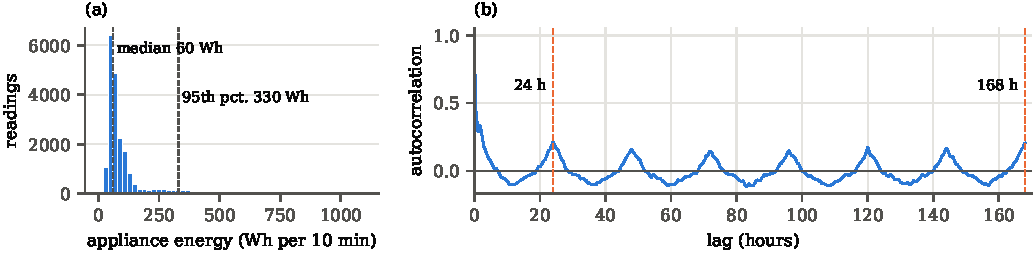
\includegraphics[width=\textwidth]{figures/fig_data.pdf}
\caption{UCI appliance energy. (a) The distribution is right-skewed (skewness 3.39): the median is 60\,Wh per
10 minutes, but the top 10\% of readings hold 37.1\% of the energy. (b) Autocorrelation falls from 0.75 at lag 1
(10 minutes) to 0.02 at 6 hours, then peaks again at 24\,h (0.22) and 168\,h (0.22). The useful history is
therefore the last hour plus the same time on earlier days, not the hours in between.}
\label{fig:data}
\end{figure*}

\begin{table}[t]
\caption{Source data}
\label{tab:datastats}
\centering
\footnotesize
\begin{tabular}{@{}p{2.75cm}p{2.35cm}p{2.35cm}@{}}
\toprule
& UCI \cite{candanedo2017} & REFIT \cite{murray2017refit,rescast} \\
\midrule
Homes & 1 (Belgium) & 20 (UK) \\
Period & Jan--May 2016 & Sep 2013--Jul 2015 \\
Interval & 10 min & 15 min \\
Readings & 19{,}735 & 1{,}044{,}201 \\
Signals & appliances, lights, 9 rooms, weather & whole house \\
Mean / median (Wh) & 97.7 / 60 & 129.9 / 76 \\
Skewness & 3.39 & 4.76 \\
Energy share of top 10\% & 37.1\% & 38.6\% \\
Lag-1 autocorrelation & 0.75 & 0.68 (mean of 20 homes) \\
Licence & CC BY 4.0 & CC BY 4.0 \\
\bottomrule
\end{tabular}
\end{table}

The UCI data \cite{candanedo2017} provides the target house. Its \texttt{Appliances} column is energy in Wh per
10 minutes, so 60\,Wh is an average power of 360\,W. The other columns include lighting energy, nine room
temperature/humidity pairs and weather-station readings. Two traps are built into this data. \texttt{T6} is a sensor
outside the north wall and tracks the outdoor temperature ($r=0.97$). \texttt{rv1} and \texttt{rv2} are random
variables that the dataset's authors added on purpose to test feature selection.

REFIT \cite{murray2017refit} adds whole-house load from 20 UK homes. We use a 15-minute snapshot published on
Hugging Face \cite{rescast}. Both sources are split \emph{chronologically}. UCI: train until 20 April 2016,
validation until 8 May, test afterwards. REFIT: train until 31 January 2015, validation until 31 March, test
afterwards.

\section{Grounded Instruction Corpus}

A Python generator, written without third-party libraries, turns each reading window into question--answer
pairs. The answer is computed by code from the numbers in the question. This is the central design decision: the
model is never asked for a fact that the prompt does not contain. The exception is the two forecast tasks, whose
reference is the reading that actually came next. They are scored separately (Section~\ref{sec:eval}).
Table~\ref{tab:corpus} lists the 14 task families.

\begin{table}[t]
\caption{Task families and training examples per source (v2 corpus)}
\label{tab:corpus}
\centering
\footnotesize
\setlength{\tabcolsep}{3pt}
\begin{tabular}{@{}lp{2.75cm}rr@{}}
\toprule
Task & Question type & UCI & REFIT \\
\midrule
\task{window_stats} & highest reading, count above a level, etc. & 10{,}000 & 20{,}000 \\
\task{forecast_next} & next 10/15-min reading & 14{,}007 & 9{,}696 \\
\task{daily_profile} & sums and comparisons over 24 hourly values & 1{,}275 & 18{,}136 \\
\task{forecast_hour} & next-hour total & 7{,}994 & 7{,}224 \\
\task{spike_check} & robust anomaly flag (median/MAD) & 1{,}624 & 11{,}800 \\
\task{unanswerable} & occupancy, appliances, faults, missing sensors & 10{,}157 & -- \\
\task{room_compare} & warmest / coldest room & 10{,}000 & -- \\
\task{lights_activity} & lighting use; occupancy refusals & 7{,}998 & -- \\
\task{outdoor_weather} & dew-point spread, \texttt{T6} vs \texttt{T\_out} & 4{,}566 & -- \\
\task{units_cost} & Wh, W, kWh and cost; tariff refusals & 4{,}173 & -- \\
\task{time_features} & weekday, weekend, seconds since midnight & 1{,}545 & 1{,}773 \\
\task{false_premise} & question asserts a peak that is not there & 3{,}204 & -- \\
\task{noise_features} & \texttt{rv1}/\texttt{rv2} traps & 1{,}918 & -- \\
\task{level_classify} & low / moderate / high / peak & 1{,}273 & -- \\
\midrule
Total & train / validation / test & \multicolumn{2}{r}{148{,}363 / 23{,}734 / 28{,}238} \\
\bottomrule
\end{tabular}
\end{table}

The generator enforces the following invariants. Context windows never cross a split boundary or a gap in the time
grid. Thresholds come from training data only. Yes/no tasks are balanced 50/50. Every prompt is unique across the
corpus; 351 prompts that mapped to two different answers were dropped. An assertion checks that no prompt appears in
more than one split. Each REFIT prompt carries a one-line house profile (median and 90th percentile from that home's
training period). Without that line, ``is this high?'' would be ill-posed across 20 different homes.

Generation is seeded and reproducible. The v1 corpus (UCI only, 2{,}500 training examples per task) has 33{,}916
pairs. The v2 corpus (10{,}000 per task plus REFIT) has 200{,}335 pairs and 25.6M training tokens. A training
sequence averages 172 tokens and is at most 415 tokens long.

\section{Model and Training}

\begin{figure}[t]
\centering
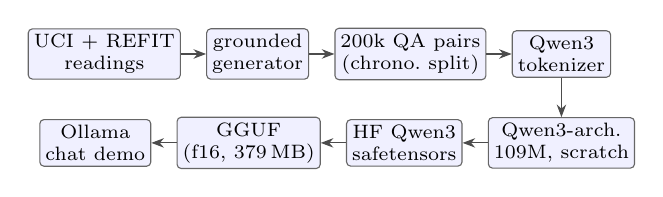
\begin{tikzpicture}[
  node distance=3.2mm, font=\scriptsize,
  box/.style={draw=black!60, rounded corners=1.5pt, fill=blue!6, align=center, minimum height=5.5mm, inner sep=2pt},
  arr/.style={-{Stealth[length=1.6mm]}, black!70}]
\node[box] (raw) {UCI + REFIT\\readings};
\node[box, right=of raw] (gen) {grounded\\generator};
\node[box, right=of gen] (corp) {200k QA pairs\\(chrono.\ split)};
\node[box, right=of corp] (tok) {Qwen3\\tokenizer};
\node[box, below=5mm of tok] (model) {Qwen3-arch.\\109M, scratch};
\node[box, left=of model] (hf) {HF Qwen3\\safetensors};
\node[box, left=of hf] (gguf) {GGUF\\(f16, 379\,MB)};
\node[box, left=of gguf] (oll) {Ollama\\chat demo};
\draw[arr] (raw) -- (gen); \draw[arr] (gen) -- (corp); \draw[arr] (corp) -- (tok); \draw[arr] (tok) -- (model);
\draw[arr] (model) -- (hf); \draw[arr] (hf) -- (gguf); \draw[arr] (gguf) -- (oll);
\end{tikzpicture}
\caption{Pipeline from raw readings to the chat demonstration.}
\label{fig:pipeline}
\end{figure}

\textbf{Architecture.} The model follows the Qwen3 decoder \cite{qwen3}. It uses grouped-query attention
\cite{ainslie2023gqa} with RMS normalisation of each query and key head, SwiGLU feed-forward layers
\cite{shazeer2020glu}, pre-normalisation with RMSNorm \cite{zhang2019rmsnorm}, and rotary position embeddings
\cite{su2024roformer} (Table~\ref{tab:arch}). Input and output embeddings are tied. The tokenizer is Qwen3's
byte-level BPE. We use its full length of 151{,}669 entries, because the reference notebook's \texttt{vocab\_size}
of 151{,}643 omits the chat special tokens. The embedding table therefore holds 77.7M of the 109.1M parameters.

\begin{table}[t]
\caption{Model and training configuration}
\label{tab:arch}
\centering
\footnotesize
\begin{tabular}{@{}p{3.25cm}p{5.05cm}@{}}
\toprule
Layers / width / FFN width & 8 / 512 / 2{,}048 \\
Attention heads / KV groups / head dim. & 8 / 4 / 64 \\
Context / RoPE base & 448 tokens / 10{,}000 \\
Parameters & 109.1M (77.7M embeddings) \\
Vocabulary & 151{,}669 (Qwen3-8B tokenizer) \\
Optimiser & AdamW \cite{loshchilov2019adamw}, $\beta=(0.9, 0.95)$, wd 0.1 \\
Learning rate & $3\!\times\!10^{-4}$, 300 warm-up updates, cosine to $3\!\times\!10^{-5}$ \cite{loshchilov2017sgdr} \\
Batch & 8 sequences $\times$ 4 accumulation steps \\
Steps (v1 / v2) & 24{,}000 / 72{,}000 batches \\
Precision & fp32 weights, bf16 autocast, gradient clip 1.0 \\
Hardware & 1$\times$ RTX 5060 Laptop (8\,GB), Ryzen 7 250 \\
Training time (v2) & 96.8 min, peak 4.6\,GiB \\
\bottomrule
\end{tabular}
\end{table}

\textbf{Loss on answers only.} Each batch holds whole examples in the chat format
\texttt{<|im\_start|>user \ldots<|im\_end|> <|im\_start|>assistant \ldots<|im\_end|>}. Padding and prompt positions
are masked, so the cross-entropy is computed on answer tokens alone.

\textbf{Fitting an 8\,GB GPU.} With a 151{,}669-wide output layer, full-sequence logits overflowed memory at batch
sizes 32 and 16. The model therefore projects to the vocabulary only at supervised positions, in float32 outside the
autocast region. With batch size 8 and gradient accumulation of 4, peak memory was 4.6\,GiB.

\textbf{Reference-notebook corrections.} The course notebook defined variables after their first use, set a minimum
learning rate above the peak rate, and omitted the chat tokens from the vocabulary (all fixed). We also counted the
learning-rate schedule in optimiser updates rather than in batches.

\section{Evaluation Method}
\label{sec:eval}

\textbf{Sample.} From the 28{,}238 test pairs we drew, with a fixed seed, up to 200 questions from each of the 20
(task, source) groups, 3{,}956 questions in all. Both models answered the same questions with greedy decoding, so
every comparison between them is paired. v1 never saw REFIT prompts, so its REFIT scores measure transfer to unseen
homes.

\textbf{Metrics.}
\emph{Exact match} (EM) requires the whole answer to equal the reference string. It applies to the 12 task families
whose answer is computable from the prompt.
\emph{Template match} replaces every number with a placeholder before comparing. It separates wording errors from
numeric errors.
\emph{Refusal behaviour}: an answer counts as a refusal if it begins with one of the generator's refusal openings
(``That cannot be \ldots'', ``I cannot give \ldots''). Applied to the reference answers, this rule agrees with the
corpus's \texttt{answerable} flag on 100\% of the sampled questions. We report the \emph{hallucination rate} (unanswerable
questions answered anyway) and the \emph{over-refusal rate} (answerable questions refused).
\emph{Forecasts} are scored by mean absolute error (MAE) of the predicted Wh against the actual next reading. They
are compared with persistence (the last reading, or the last hour for next-hour totals) and with the window mean
\cite{hyndman2021fpp3}.

\textbf{Statistics.} Proportions carry Wilson 95\% intervals \cite{wilson1927}. v1 and v2 are compared with the
exact McNemar test on discordant pairs \cite{mcnemar1947}. Paired forecast errors are compared with the Wilcoxon
signed-rank test \cite{wilcoxon1945}, and the mean error difference carries a 10{,}000-sample bootstrap 95\%
interval \cite{efron1979}. The effect of prompt length is measured by the point-biserial correlation between
correctness and the count of numbers in the prompt, and by a one-sided Mann--Whitney test. UCI and REFIT are compared
on shared tasks with Fisher's exact test. The significance level is $\alpha=0.05$; per-task tests are reported
without multiplicity correction and should be read as descriptive.

\section{Results}

\subsection{Training dynamics}

\begin{figure}[t]
\centering
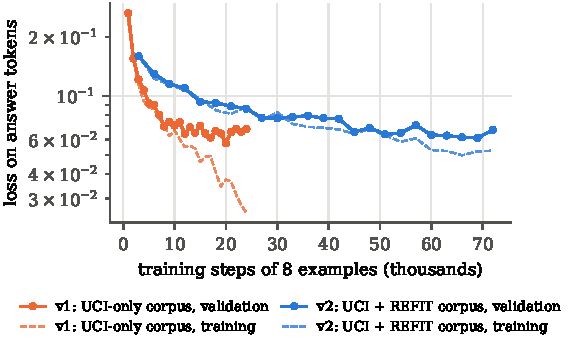
\includegraphics[width=\columnwidth]{figures/fig_loss.pdf}
\caption{Training and validation loss on answer tokens. v1 (UCI-only corpus, 7.7 epochs) overfits: its training
loss falls to 0.025 while validation loss stalls near 0.068. v2 (3.9 epochs over a 5.9$\times$ larger corpus) keeps
the two curves within 0.015 of each other. The validation sets differ, so absolute values are not comparable across
runs.}
\label{fig:loss}
\end{figure}

Fig.~\ref{fig:loss} shows both runs. v1 saw 192k examples, 7.7 passes over its 25{,}027 training pairs. Its
training loss kept falling to 0.025, while validation loss levelled off at about 0.07 after step 10{,}000 (best 0.0574
at step 20{,}000). v2 saw 576k examples, 3.9 passes over 148{,}363 pairs. Its final training and validation losses
were 0.053 and 0.067 (best validation 0.0611 at step 69{,}000), so the larger corpus removed most of the
generalisation gap.

\subsection{Exact match}

\begin{table*}[t]
\caption{Exact match (\%) on held-out test questions. Both models answered the same questions. CI: Wilson 95\%
interval for v2. Template: \% of v2 answers whose wording is right once numbers are masked. $p$: exact McNemar
test, v1 vs v2.}
\label{tab:em}
\centering
\footnotesize
\begin{tabular}{@{}llrrrcrr@{}}
\toprule
Task & Source & $n$ & v1 & v2 & 95\% CI (v2) & Template (v2) & $p$ \\
\midrule
daily\_profile & REFIT & 200 & 1.5 & \textbf{14.5} & [10.3, 20.0] & 92.0 & $<$0.001 \\
daily\_profile & UCI & 200 & 0.0 & \textbf{5.0} & [2.7, 9.0] & 92.0 & 0.002 \\
false\_premise & UCI & 200 & 98.0 & \textbf{100.0} & [98.1, 100.0] & 100.0 & 0.125 \\
level\_classify & UCI & 156 & 100.0 & \textbf{100.0} & [97.6, 100.0] & 100.0 & 1.000 \\
lights\_activity & UCI & 200 & 100.0 & \textbf{100.0} & [98.1, 100.0] & 100.0 & 1.000 \\
noise\_features & UCI & 200 & 100.0 & \textbf{100.0} & [98.1, 100.0] & 100.0 & 1.000 \\
outdoor\_weather & UCI & 200 & 21.5 & \textbf{25.0} & [19.5, 31.4] & 99.5 & 0.167 \\
room\_compare & UCI & 200 & 45.0 & \textbf{46.5} & [39.7, 53.4] & 73.5 & 0.743 \\
spike\_check & REFIT & 200 & 5.0 & \textbf{45.0} & [38.3, 51.9] & 99.5 & $<$0.001 \\
spike\_check & UCI & 200 & 15.5 & \textbf{38.5} & [32.0, 45.4] & 97.5 & $<$0.001 \\
time\_features & REFIT & 200 & 11.5 & \textbf{61.5} & [54.6, 68.0] & 61.5 & $<$0.001 \\
time\_features & UCI & 200 & 50.5 & \textbf{87.5} & [82.2, 91.4] & 87.5 & $<$0.001 \\
unanswerable & UCI & 200 & 100.0 & \textbf{100.0} & [98.1, 100.0] & 100.0 & 1.000 \\
units\_cost & UCI & 200 & 95.0 & \textbf{95.5} & [91.7, 97.6] & 100.0 & 1.000 \\
window\_stats & REFIT & 200 & 13.0 & \textbf{51.5} & [44.6, 58.3] & 95.0 & $<$0.001 \\
window\_stats & UCI & 200 & 18.0 & \textbf{37.0} & [30.6, 43.9] & 95.0 & $<$0.001 \\
\midrule
\textit{pooled} & UCI & 2356 & 61.2 & \textbf{69.0} & [67.1, 70.9] & 95.3 & $<$0.001 \\
\textit{pooled} & REFIT & 800 & 7.8 & \textbf{43.1} & [39.7, 46.6] & 87.0 & $<$0.001 \\
\bottomrule
\end{tabular}
\end{table*}

\begin{figure}[t]
\centering
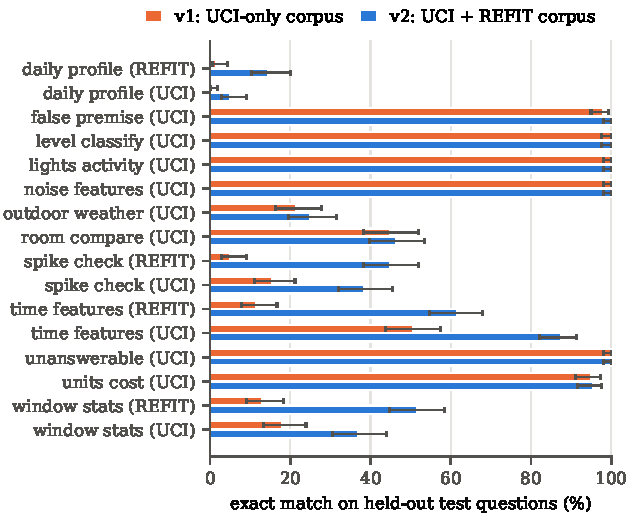
\includegraphics[width=\columnwidth]{figures/fig_exact_match.pdf}
\caption{Exact match per task and source with Wilson 95\% intervals.}
\label{fig:em}
\end{figure}

Table~\ref{tab:em} and Fig.~\ref{fig:em} give exact match for the 12 computable task families. On the 2{,}356 UCI
questions, v2 reached 69.0\% [67.1, 70.9] against 61.2\% for v1. Of the discordant pairs, v2 alone was right on 216
and v1 alone on 33 ($p=3.9\times10^{-34}$). On the 800 REFIT questions the gain was 7.8\% $\rightarrow$ 43.1\%
(286 vs.\ 3 discordant pairs, $p=8.1\times10^{-81}$). REFIT measures transfer for v1, which never saw those homes;
for v2 it measures held-out \emph{future} periods of homes it was trained on.

The gains concentrate in the tasks that the larger corpus fed most. For UCI \task{spike_check}, \task{time_features}
and \task{window_stats}, accuracy rose by 19--37 points ($p<0.001$). The six symbolic tasks (\task{false_premise},
\task{level_classify}, \task{lights_activity}, \task{noise_features}, \task{unanswerable}, \task{units_cost}) were
already at 95--100\% in v1 and stayed there. Two tasks remain weak. \task{daily_profile} reached only 5.0\% on UCI and
14.5\% on REFIT; it asks for sums of up to 24 four-digit values. \task{outdoor_weather} reached 25.0\%. Its wrong answers have the right wording (99.5\% template match), but a
temperature difference or dew-point spread is off by 0.1--0.6\,\textdegree C.

\subsection{Refusals and hallucination}

\begin{table*}[t]
\caption{Refusal behaviour over all sampled questions. TP: unanswerable and refused; FN: unanswerable but answered
(hallucination); FP: answerable but refused; TN: answerable and answered. Rates in \% with Wilson 95\% intervals.}
\label{tab:refusal}
\centering
\footnotesize
\begin{tabular}{@{}lrrrrrrcc@{}}
\toprule
Model (questions) & TP & FN & FP & TN & Precision & Recall & Hallucination rate & Over-refusal rate \\
\midrule
v1 (UCI questions) & 364 & 0 & 0 & 2392 & 100.0 & 100.0 & 0.0 [0.0, 1.0] & 0.0 [0.0, 0.2] \\
v2 (UCI questions) & 364 & 0 & 0 & 2392 & 100.0 & 100.0 & 0.0 [0.0, 1.0] & 0.0 [0.0, 0.2] \\
v2 (all questions) & 364 & 0 & 0 & 3592 & 100.0 & 100.0 & 0.0 [0.0, 1.0] & 0.0 [0.0, 0.1] \\
\bottomrule
\end{tabular}
\end{table*}

Both models refused every one of the 364 unanswerable questions and none of the answerable ones
(Table~\ref{tab:refusal}). For v2, the 95\% upper bounds are 1.0\% for the hallucination rate and 0.1\% for the
over-refusal rate. False-premise questions (``the appliances peaked at 900\,Wh; what caused it?'') were rejected in
100\% of cases. This is the most direct outcome of the design-thinking work: the missing-labels problem from the
Define stage became a corpus invariant, and the trained model kept to it.

\subsection{Error analysis}

\begin{figure}[t]
\centering
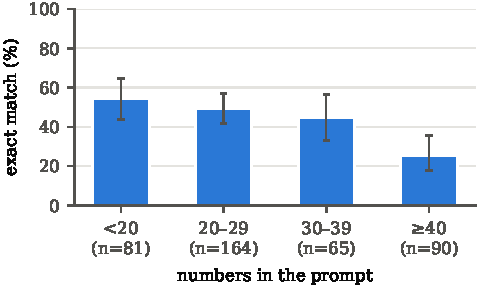
\includegraphics[width=\columnwidth]{figures/fig_numbers.pdf}
\caption{Exact match on \task{window_stats} (UCI and REFIT, $n=400$) against the count of numbers in the prompt,
with Wilson 95\% intervals.}
\label{fig:numbers}
\end{figure}

v2 answered 1{,}185 computable questions wrongly. In 971 of them (81.9\%), the answer matched the reference once
numbers were masked: the model chose the right answer form and got a number wrong. Nearly all the remaining 214 are
categorical results computed from the prompt, not refusals: a wrong weekday (102), a wrong room (53), or a wrong list
of hours above a threshold (32). No error involved a wrong refusal or a missed one.

Arithmetic degrades with the amount of numeric evidence. Within one task, \task{window_stats}, correct answers had
a median of 24 numbers in the prompt and wrong answers 29. The point-biserial correlation between correctness and
number count is $r=-0.21$ ($p=1.5\times10^{-5}$; one-sided Mann--Whitney $p=1.1\times10^{-4}$). Accuracy falls from
54.3\% below 20 numbers to 25.6\% at 40 or more (Fig.~\ref{fig:numbers}). The Qwen3 tokenizer splits every number
into digits, so a 24-value sum is a long chain of digit-level operations for a 109M model. This matches the
tokenisation problem anticipated in the Define stage, and earlier observations on digit tokenisation in LLMs
\cite{gruver2023llmtime}.

Data volume matters per task. REFIT \task{daily_profile} had 14$\times$ more training pairs than UCI
\task{daily_profile} (18{,}136 vs.\ 1{,}275) and scored higher (14.5\% vs.\ 5.0\%, Fisher $p=0.002$). The same holds
for \task{window_stats} (20{,}000 vs.\ 10{,}000 pairs; 51.5\% vs.\ 37.0\%, $p=0.005$). The exception is
\task{time_features}: with similar counts, REFIT scored lower (61.5\% vs.\ 87.5\%, $p<0.001$). A weekday cannot be
read off the prompt; it has to be derived from the calendar date. A plausible cause is that the REFIT test dates
(2015) lie further from most of their training dates (2014) than the UCI test dates do from theirs.

\subsection{Forecasting}

\begin{table*}[t]
\caption{Forecast mean absolute error (Wh). Persistence repeats the last reading (or the last hour); the window mean
repeats the prompt's average. $\Delta$: model minus persistence with bootstrap 95\% interval. $p$: Wilcoxon
signed-rank test, model vs.\ persistence. Skill: $1-\mathrm{MAE}_{\text{model}}/\mathrm{MAE}_{\text{persistence}}$.}
\label{tab:forecast}
\centering
\footnotesize
\begin{tabular}{@{}llrrrrrcrr@{}}
\toprule
Task & Source & $n$ & v2 & v1 & Persistence & Window mean & $\Delta$ [95\% CI] & $p$ & Skill \\
\midrule
forecast\_next & UCI & 200 & \textbf{28.4} & 31.5 & 31.8 & 35.5 & -3.4 [-9.6, +2.9] & 0.043 & +0.11 \\
forecast\_next & REFIT & 200 & \textbf{39.4} & -- & 33.4 & 46.9 & +6.0 [+0.4, +12.1] & 0.065 & -0.18 \\
forecast\_hour & UCI & 200 & \textbf{185.4} & 196.4 & 195.5 & 188.8 & -10.1 [-37.1, +16.4] & 0.956 & +0.05 \\
forecast\_hour & REFIT & 200 & \textbf{202.4} & -- & 189.4 & 204.5 & +13.0 [-19.3, +44.1] & 0.071 & -0.07 \\
\bottomrule
\end{tabular}
\end{table*}

\begin{figure}[t]
\centering
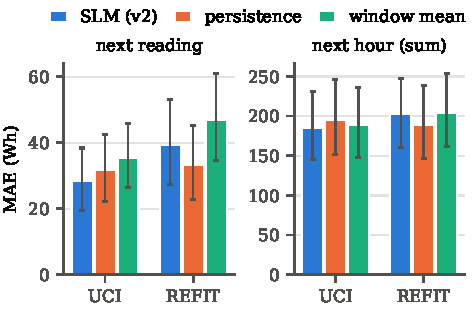
\includegraphics[width=\columnwidth]{figures/fig_forecast.pdf}
\caption{Forecast MAE with bootstrap 95\% intervals.}
\label{fig:forecast}
\end{figure}

Table~\ref{tab:forecast} and Fig.~\ref{fig:forecast} compare the forecasts with the naive baselines. No forecast
differs from persistence by a margin whose bootstrap interval excludes zero, except REFIT next-step, where the model
is \emph{worse} by 6.0\,Wh [0.4, 12.1]. On UCI next-step the model is 3.4\,Wh better, a skill of 0.11. The Wilcoxon
test is borderline ($p=0.043$), but the bootstrap interval [$-9.6$, $+2.9$] includes zero. v1 transferred poorly to
REFIT homes (next-step MAE 126.8 vs.\ 39.4\,Wh for v2).

A smaller sample would have told a different story. The training notebook's 30-question evaluation reported a
next-hour UCI MAE of 152.7\,Wh against 198.7 for persistence, a 23\% gain. On 200 questions, the gap shrinks to
185.4 vs.\ 195.5 and is not significant ($p=0.96$). We therefore report only the larger evaluation.

These results are what the autocorrelation analysis predicts. A window of 3--12 readings carries the lag-1
information that persistence already uses (Fig.~\ref{fig:data}b). The daily and weekly structure lies outside the
window, which is the gap that the project's how-might-we statement targets.

\section{Deployment and Availability}

\textbf{Conversion.} The notebook model differs from the Hugging Face \texttt{Qwen3ForCausalLM} in one respect: it
multiplies token embeddings by $\sqrt{d}$. We folded that scale into an untied input embedding and kept the unscaled
matrix as the output head. On 10 test prompts, the converted model's logits match the original to within
$1.5\times10^{-5}$. We then wrote the weights as a float16 GGUF file \cite{llamacpp} (379\,MB). The writer is a short
script using the \texttt{gguf} Python package, because the installed Ollama (v0.40) on Linux cannot import
safetensors directly.

\textbf{Chat demonstration.} An Ollama Modelfile \cite{ollama} applies the training prompt format, sends only the
latest user message (the model was trained on single questions), and decodes greedily. On one test question
from each of the 20 (task, source) groups, Ollama's answers were identical to those of the float32
\texttt{transformers} model. Measured over 20 test questions, the model generated a
median of 370 tokens/s (0.11\,s per answer) on the laptop GPU. Restricted to the Ryzen 7 250 CPU, it generated
107 tokens/s (0.58\,s per answer), fast enough for a hub without a GPU.

\textbf{Availability.} The corpus is published as the \texttt{large} configuration of the Hugging Face dataset
\url{https://huggingface.co/datasets/Design-Thinking-SLM/smart-home-energy-slm} (the original UCI-only corpus remains its default
configuration). The model (Hugging Face weights, GGUF file, Modelfile, original checkpoint, training notebook and all
evaluation answers) is published at \url{https://huggingface.co/Design-Thinking-SLM/smart-home-energy-qwen3-scratch}. The source code is
at \url{https://github.com/Ojas1004/design_thinking_slm_project}.

\section{Discussion}

\textbf{What the design process changed.} Three of the five Define-stage problems were solved by the corpus design
alone. Missing labels and misleading channels led to refusal and trap tasks, and the model handles these without
error. The single-house problem led to REFIT data, which raised REFIT exact match from 7.8\% to 43.1\% and also
improved the UCI house. Number tokenisation remains the binding constraint, and heavy-tailed peaks remain
unforecastable from short windows. Both point to the HMW statement: give the model the right numbers (same time
yesterday and last week) instead of more of them.

\textbf{Threats to validity.}
(i) The questions are generated from templates. The test set measures generalisation to new readings and later
periods, not to new phrasings; free-form questions fail.
(ii) Exact match is strict. A sum off by 10\,Wh counts as wrong. The template-match column separates such errors.
(iii) v1 and v2 differ in corpus size, task mix and training length. The comparison measures the whole data
intervention, not corpus size alone.
(iv) Each model was trained once, with one seed.
(v) Per-task tests are uncorrected. Under a Bonferroni correction across the 16 exact-match comparisons
($\alpha=0.003$), the pooled results and every per-task difference reported with $p<0.001$ remain significant.

\textbf{Future work.} Route arithmetic to code: the model chooses the operation and a tool computes it. Add
retrieved lag readings (same time yesterday and last week) to forecast prompts, following HMW~1. Compare training
from scratch with LoRA fine-tuning \cite{hu2022lora} of a pretrained model of similar size.

\section{Conclusion}

Design thinking turned an exploratory look at one house's meter data into concrete rules for a training corpus.
Those rules produced a 109M-parameter model, trained from scratch on a laptop, that never invented an answer to an
unanswerable question in 3{,}956 test cases. It answers symbolic questions almost perfectly and runs in under a
second on a CPU. Its limits are equally clear: multi-number arithmetic and forecasting beyond persistence. Both are
problems of what the model is given to read, not of how large it is, and they define the next iteration.

\section*{Acknowledgment}

The authors thank Dr.\ Sujeet S.\ Jagtap for guidance in the Design Thinking course (25ESHS01) at Jain University,
and the creators of the UCI Appliances Energy Prediction and REFIT datasets for releasing them under open licences.

\bibliographystyle{IEEEtran}
\bibliography{refs}

\end{document}
